\documentclass[12pt,letterpaper]{article}

\title{HoraDelCódigo™ en UTFSM}

\usepackage[english]{babel}
\usepackage[utf8]{inputenc}
\usepackage[sfdefault,lf]{carlito}

\usepackage[margin=1.1cm,letterpaper]{geometry}
\usepackage{multicol}
\usepackage{ragged2e}
\usepackage{tabularx}
\usepackage[table]{xcolor}
\usepackage{graphicx}

\definecolor{OverleafGreen}{HTML}{4F9C45}
\definecolor{celesteletras}{HTML}{1AADBB}
\definecolor{celeste}{HTML}{7FD8DF}
\graphicspath{{images/}}
\pagestyle{empty}
\RaggedRight
\parskip=12pt plus 4pt

\begin{document}

{\fontsize{38pt}{40pt}\bfseries\selectfont\color{celeste}
Participa de la HoraDelCódigo 2018
\par}

\begin{multicols}{2}

{\LARGE\bfseries
\mbox{En la UTFSM Campus San Joaquín!\par}
}

{\Large
Se parte de una de las convocatorias más grandes del mundo para acercar las Ciencias de la Computación a los jóvenes!
\par}

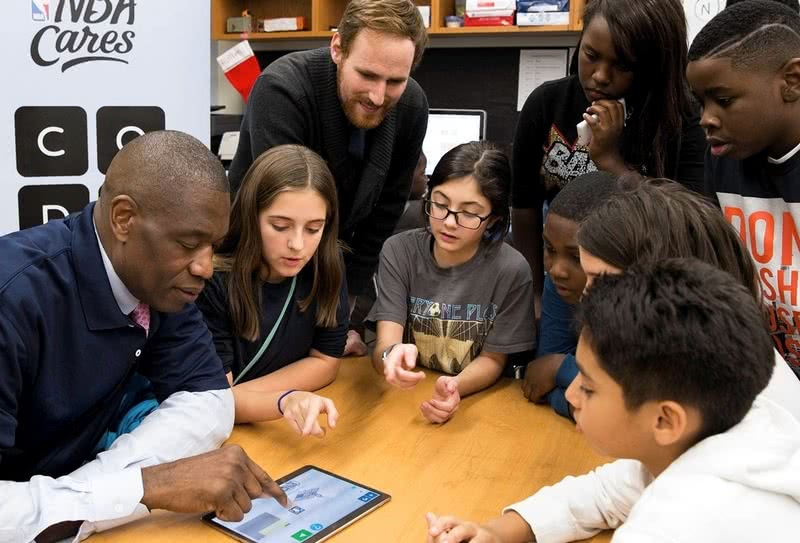
\includegraphics[width=\linewidth]{highlight-nba}

\columnbreak
\setlength{\leftskip}{40pt}
{\centering

\includegraphics[width=.55\linewidth]{logo}
\par}

\textbf{Qué es?} La HoraDelCódigo es una introducción de una hora a la informática, diseñada para desmitificar la programación y demostrar que cualquiera puede aprender los conceptos básicos.\par

\textbf{Qué se hace?} En LaHoraDelCódigo tendrás la oportunidad de  desarrollar una de las actividades preparadas especialmente para entregar un real acercamiento a las Ciencias de la Computación así como pasar un rato divertido, bajo la guía de tutores expertos en el área.\par

\end{multicols}

\vskip -\baselineskip
\hskip -1.1cm
\renewcommand{\arraystretch}{1.8}
\begin{tabularx}{\paperwidth}{
   @{} p{1.5cm} @{}
   *4{>{\centering\arraybackslash\large\bfseries}X @{}}
   p{1.5cm} @{}
}
\rowcolor{celeste}
\rule{0pt}{2.2cm} & 

\includegraphics[height=1.8cm]{green_light_bulb} &

\includegraphics[height=1.8cm]{projector_screen} &

\includegraphics[height=1.8cm]{Globe_Mouse} &

\includegraphics[height=1.8cm]{pencil-308509} & \\[0.1cm]
& Desarrolla & Investiga & Comparte & Aprende &\\
\end{tabularx}


\begin{large}
\textbf{Como me inscribo?} En desarrollo. . . . . . . . . . . . . . . . . . . . . . . . . . . . . . . . . . . . . . . . . . . . . . . . . . . . . . . . . . . . . . . . . . . . . . . . . . . . . . . . . . . . . . . . . . . . . . . . . . . . . . . . . . . . . . . . . . . . . . . . . . . . . . . . . . . . . . . . . . . . . . . . . . . . . . . . . . . . . . . . . . . . . . . . \par

\textbf{Donde?} En la Universidad Técnica Federico Santa María -- Campus San Joaquín, Avda. Vicuña Mackenna 3939, San Joaquín, Santiago.\par

\textbf{Otros:} En desarrollo. . . . . . . . . . . . . . . . . . . . . . . . . . . . . . . . . . . . . . . . . . . . . . . . . . . . . . . . . . . . . . . . . . . . . . . . . . . . . . . . . . . . . . . . . . . . . . . . . . . . . . . . . . . . . . . . . . . . . . . . . . . . . . . . . . . . . . . . . . . . . . . . . . . . . . . . . . . . . . . . . . . . . . . .  (comida)\par
\end{large}

\vfill

\includegraphics[width=7cm]{logou}
\hfill

\includegraphics[width=1.3cm]{logo}
\end{document}